\section{Competing Applications}
\label{sec:competition}
With work and school continuing online, it is more common now to have multiple applications simultaneously using the home network, potentially leading to competition between any combination of VCAs, video streaming, or other popular applications. In this section, we measure how VCAs perform in the presence of other applications sharing the same bottleneck link. Specifically, we focus on link sharing with other VCAs, a single TCP flow (iPerf3), and two popular video streaming applications, Netflix and YouTube (uses QUIC). 


\begin{figure}[t!]
\centering
\begin{subfigure}[t]{.5\textwidth}
    \centering
    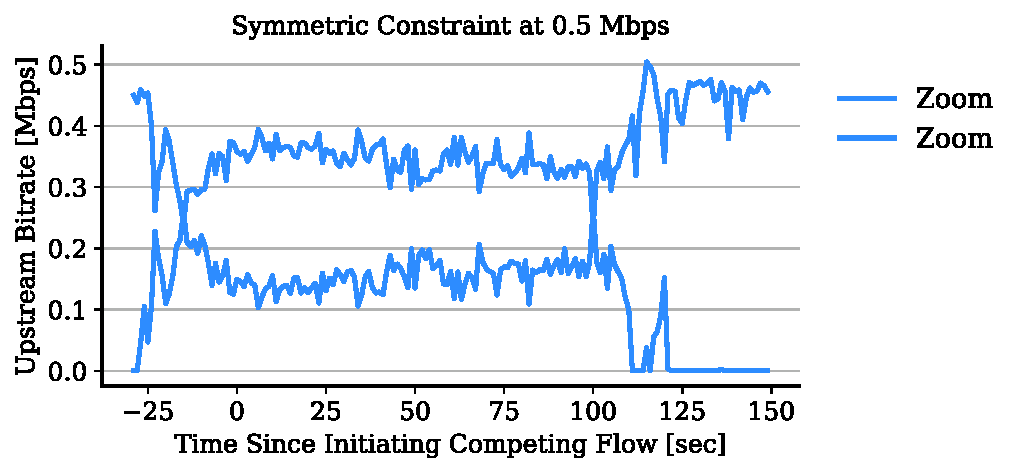
\includegraphics[width=1\textwidth]{comp/zoom_vs_zoom_0_5.pdf}
    \caption{Zoom}
    \label{fig:zoom_box_1}
\end{subfigure}\hfill
\begin{subfigure}[t]{.5\textwidth}
    \centering
    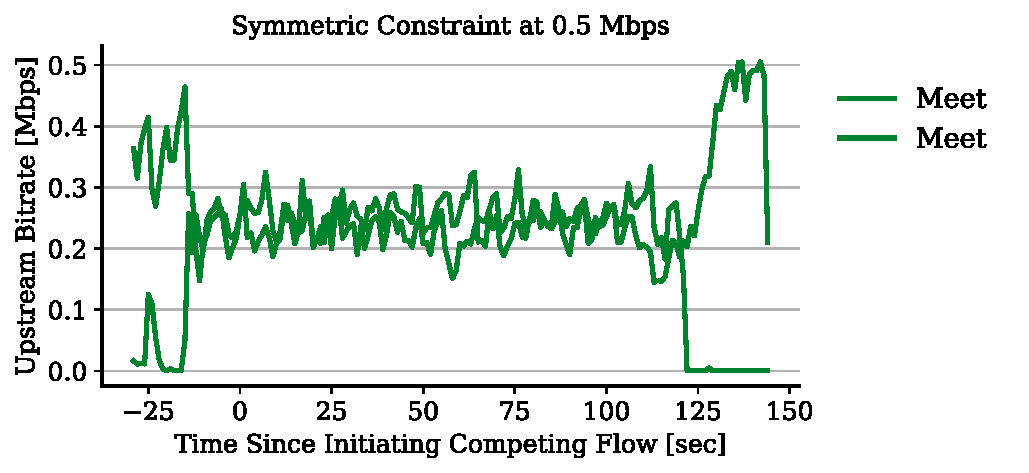
\includegraphics[width=1\textwidth]{figures/comp/meet_vs_meet_0_5.pdf}
    \caption{Meet}
    \label{fig:zoom_box_1}
\end{subfigure}
\caption{Upstream utilization of competition between Zoom/Zoom and Meet/Meet}
\label{fig:meet-zoom-upld-0.5}
\end{figure}

\begin{figure*}[t!]
\centering
\begin{subfigure}[t]{.33\textwidth}
    \centering
    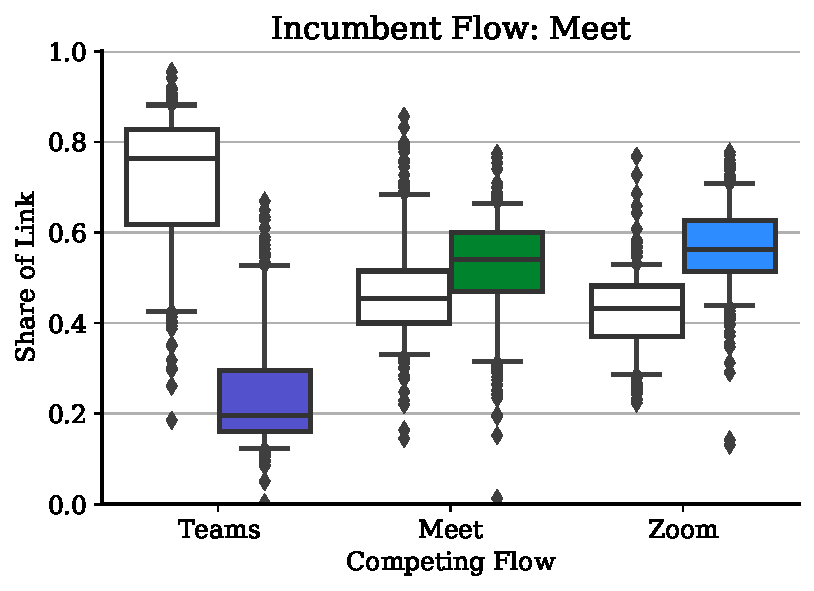
\includegraphics[width=1\textwidth]{figures/comp_all/box_plot_meet_dl_0.5_all.pdf}
    \caption{Meet}
    \label{fig:meet-dl-boxplot-0.5}
\end{subfigure}\hfill
\begin{subfigure}[t]{.33\textwidth}
    \centering
    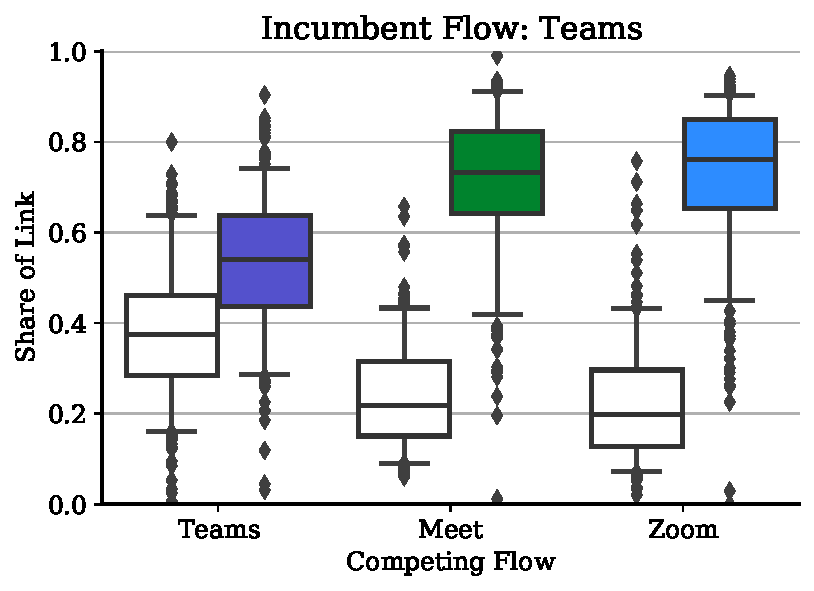
\includegraphics[width=1\textwidth]{figures/comp_all/box_plot_teams_dl_0.5_all.pdf}
    \caption{Teams}
    \label{fig:teams-dl-boxplot-0.5}
\end{subfigure}
\begin{subfigure}[t]{.33\textwidth}
    \centering
    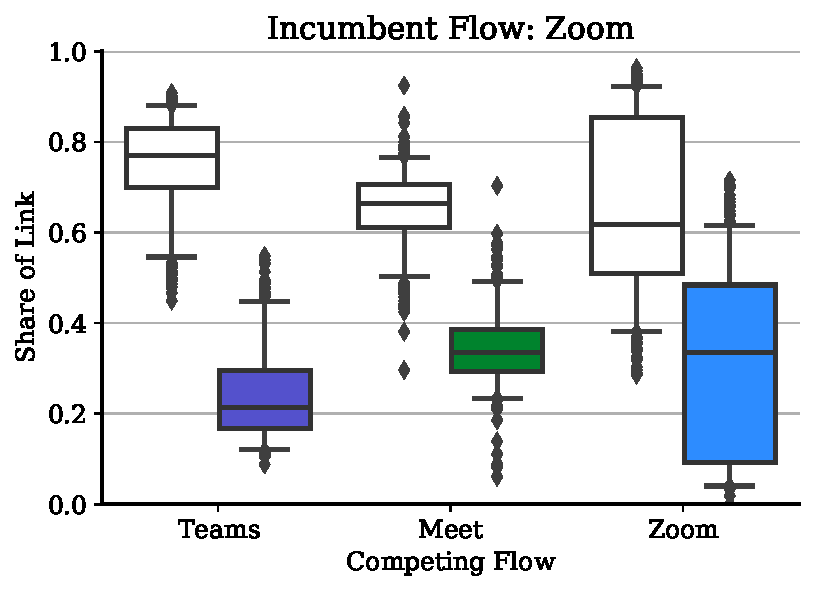
\includegraphics[width=1\textwidth]{figures/comp_all/box_plot_zoom_dl_0.5_all.pdf}
    \caption{Zoom}
    \label{fig:zoom-dl-boxplot-0.5}
\end{subfigure}
\caption{Downstream bitrate of applications in competition with each VCA, with a link shaped symmetrically at 0.5~Mbps.}
\label{fig:dnld-boxplot}
\end{figure*}

\begin{figure}[t!]
\centering
\begin{subfigure}[t]{.5\textwidth}
    \centering
    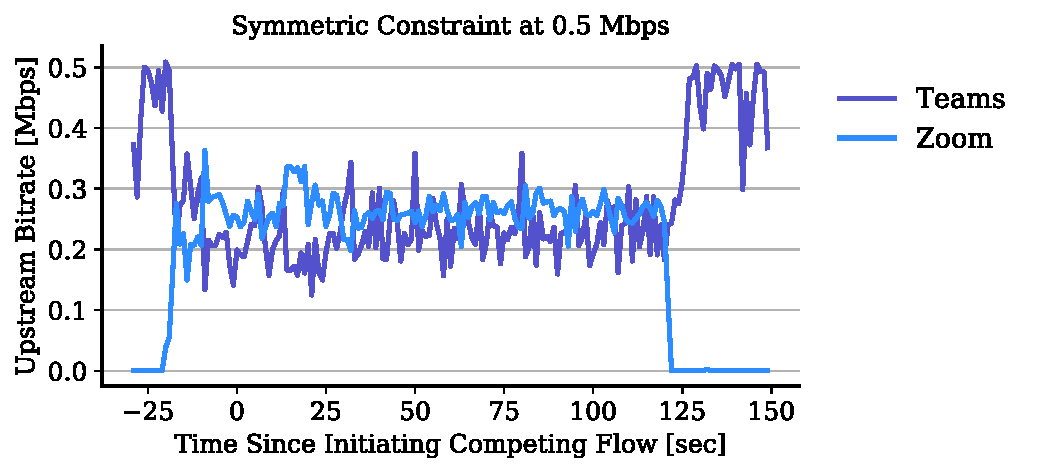
\includegraphics[width=1\textwidth]{figures/comp/teams_vs_zoom_up_1.pdf}
    \caption{Zoom}
    \label{fig:teams-zoom-up-1}
\end{subfigure}\hfill
\begin{subfigure}[t]{.5\textwidth}
    \centering
    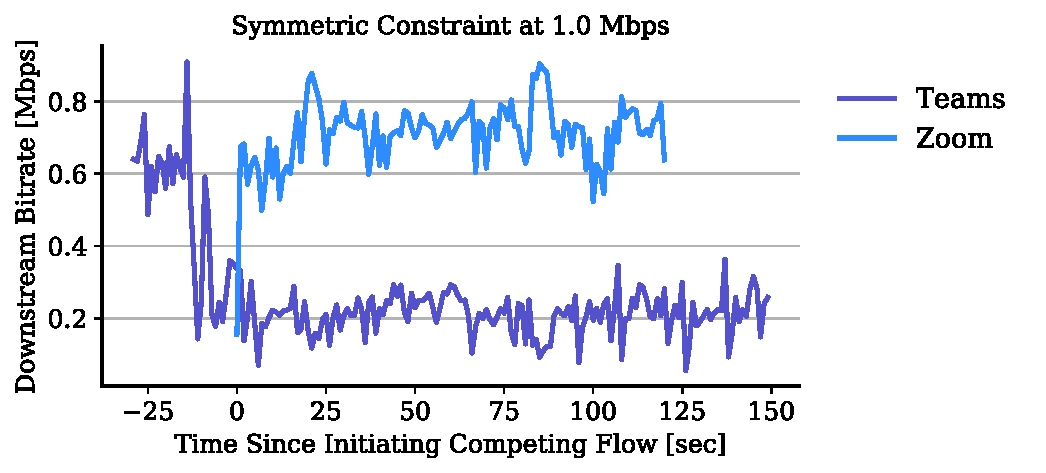
\includegraphics[width=1\textwidth]{figures/comp/teams_vs_zoom_down_1.pdf}
    \caption{Meet}
    \label{fig:teams-zoom-down-1}
\end{subfigure}
\caption{Comparison of Teams competition behavior in the uplink and downlink}
\label{fig:teams-zoom-1}
\end{figure}


\noindent \textbf{Methodology}: As illustrated in Figure \ref{fig:competition-setup}, the setup for these experiments differs slightly from earlier ones. 
Instead of connecting the client directly to the router, the two matched clients, C1 and F1, are connected to the router via a switch. 
The link between the switch and the router is shaped by the router. For each test, C1 first establishes a VCA call with C2.
Approximately 30 seconds later, F1 establishes a competing flow, which lasts for two minutes.
F1's counter-party, F2, depends on the type of flow.
If the competing flow is a VCA call, then F2 is another consumer laptop.
If the competing flow is an iPerf3 (TCP) flow, then F2 is a server on the same network,
  and if the flow is Netflix or Youtube, then F2 is a server for the respective service. Netflix and Youtube are launched directly in Chrome via \texttt{xdg-open}.
After the competing flow terminates, the incumbent flow continues for an additional minute.
We repeat each experiment with bandwidth shaped symmetrically at \{0.5, 1, 2, 3, 4, 5\}~Mbps.

\subsection{VCA vs VCA}


\begin{figure}[t!]
\centering
\begin{subfigure}[t]{.23\textwidth}
    \centering
    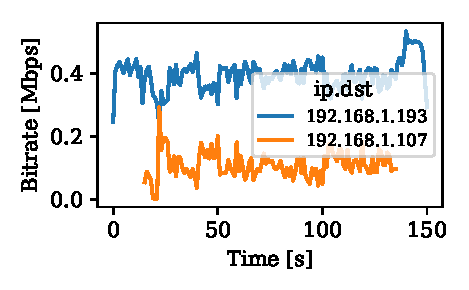
\includegraphics[width=1\textwidth]{figures/comp/zoom_netflix_timeseries.pdf}
    \caption{Downlink bitrate for Zoom and Netflix}
    \label{fig:comp_zoom_netflix_bitrate}
\end{subfigure}\hfill
\begin{subfigure}[t]{.23\textwidth}
    \centering
    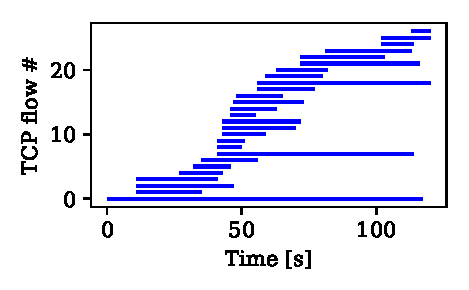
\includegraphics[width=1\textwidth]{figures/comp/netflix_connection_0_5.pdf}
    \caption{TCP connections opened by Netflix}
    \label{subfig:comp_netflix_conn}
\end{subfigure}
\caption{Zoom vs Netflix on a 0.5 Mbps downlink}
\label{fig:comp_netflix_zoom}
\end{figure}

We first analyze link sharing between each possible pair of the three VCAs under different symm  
We find that VCAs are able to achieve their nominal bitrate when the link capacity is 4 Mbps or higher. This is expected as the link capacity exceeds the sum of nominal bitrates of each VCAs. We then focus on the region, when the link capacity is lower, leading to competition between the VCAs. Given that there are only two competing clients, we use the proportion of the link shared as a metric to assess fairness. A VCA is termed as aggressive, if it uses more than half of the link capacity under competition, and passive otherwise.


% To study how VCAs compete, the shared link capacity must be less than a threshold defined by each application's nominal bitrate. Using Figure \ref{fig:competition-setup}, let the bottleneck bandwidth be $B$ and C1 and F1's nominal bitrate be $b_1$ and $b_2$, respectively. If $B > b_1 + b_2$, then there is enough bandwidth for both applications to operate at their nominal bitrate. When $B < b_1 + b_2$, the applications must compete over limited bandwidth. We define fairness in competition to be when an application uses half of the available bandwidth. We say that an application is aggressive if it uses more than half and passive if it uses less. 


When there are simultaneous VCAs on the same network, there will be competition on both the uplink and downlink.
Looking first at the uplink, we observe differences in how each VCA shares the link. Figure \ref{fig:boxplot-upld} shows how Meet and Teams tend to share the link fairly with all other VCAs while Zoom aggressively consumes close to $75\%$ of the available bandwidth. Interestingly, Zoom even behaves unfairly with other Zoom flows, suggesting that the incumbent Zoom application prioritizes itself regardless of the competing application. 


Turning to downlink sharing, Meet and Teams no longer consistently behave fairly. Meet consumes over $75\%$ of the downlink bandwidth when competing with Teams. Conversely, Teams backs off when competing with Meet and Zoom. This asymmetrical response is exemplified in Figure X, which compares how Teams competes with Meet on the uplink vs. the downlink. 



The way each VCA shares the link with other applications is made clear in Figure \ref{fig:dnld-boxplot}. We see that Zoom uses well over $50\%$ of the available capacity against other VCA.

\begin{figure}[t!]
\centering
\begin{subfigure}[t]{.23\textwidth}
    \centering
    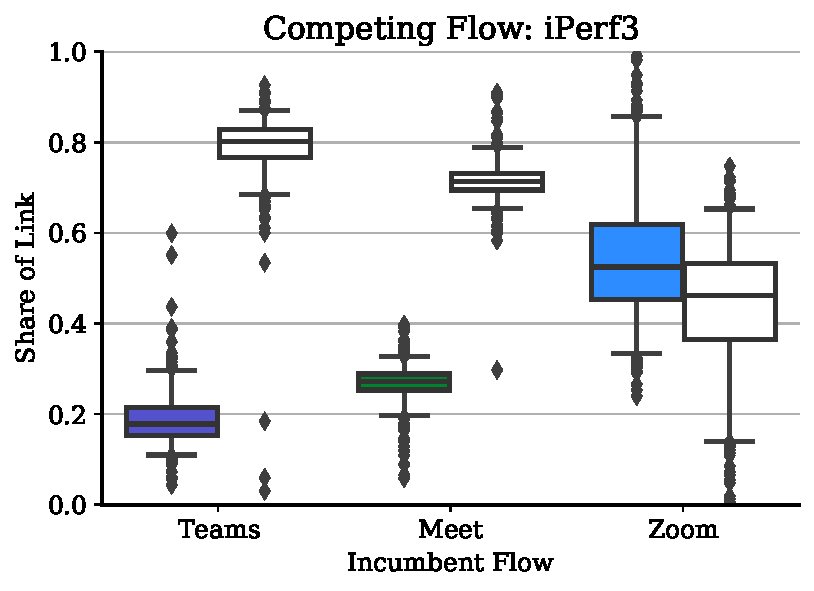
\includegraphics[width=1\textwidth]{figures/comp_all/box_plot_iperf_dl_2.0_all.pdf}
    \caption{Downlink}
    \label{fig:boxplot-iperf-dl}
\end{subfigure}\hfill
\begin{subfigure}[t]{.23\textwidth}
    \centering
    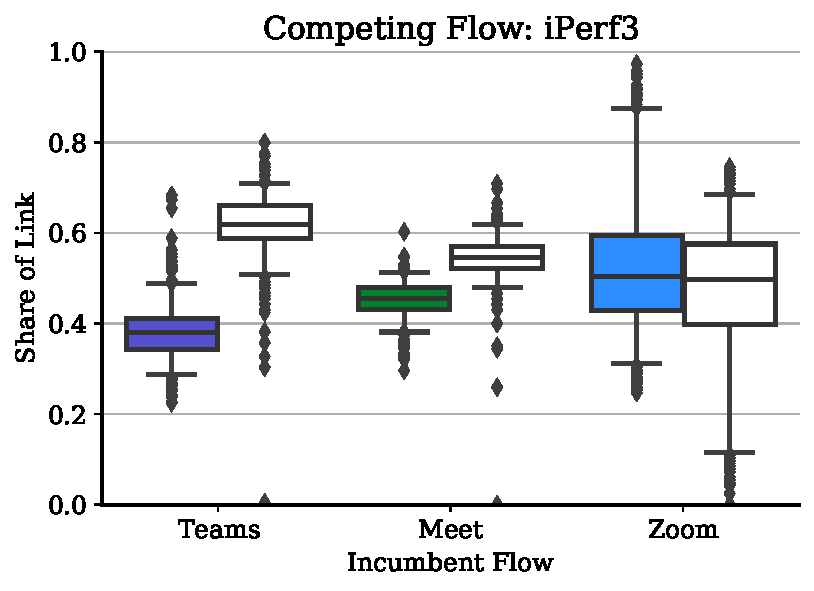
\includegraphics[width=1\textwidth]{figures/comp_all/box_plot_iperfup_ul_2.0_all.pdf}
    \caption{Uplink}
    \label{subfig:boxplot-iperf-ul}
\end{subfigure}
\caption{iPerf3 link sharing with VCAs}
\label{fig:boxplot-iperf}
\end{figure}

\begin{figure}[t]
    \centering
    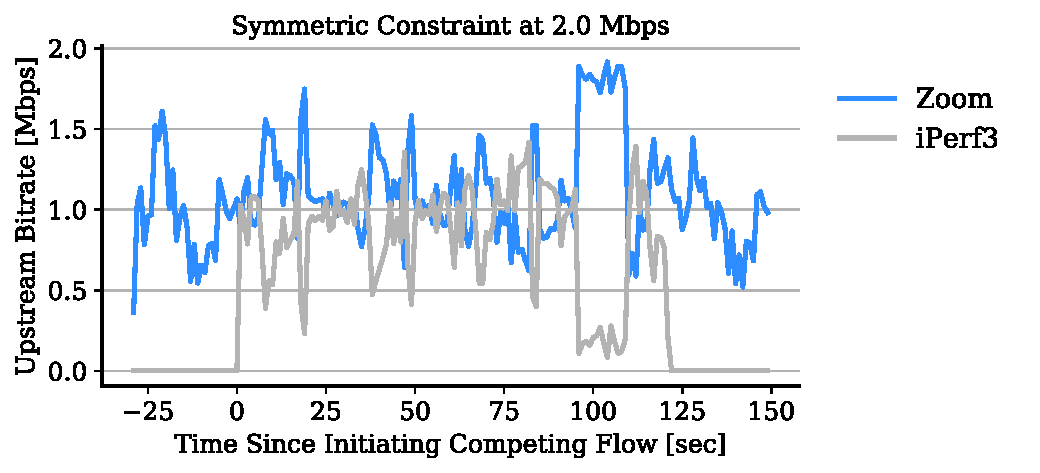
\includegraphics[width=\linewidth]{figures/comp/zoom_vs_iperf_2_down.pdf}
    \caption{Example of how Zoom probing can adversely affect competing applications}
	\label{fig:zoom-iperf-dl-2}
\end{figure}

\subsection{VCA vs TCP-flow}
We now compare how the three VCAs compete with a TCP flow. We use an iPerf3 server using TCP CUBIC and situated within the same network (RTT ~2ms) to generate the competing TCP traffic. Figure~\ref{} shows the boxplot of . Note that in all these experiments . We find two differences, Meet is even more aggressive compared to TCP during downlink competition. Teams backs off during uplink competition. Zoom behaves similarly in both directions.  

In the previous section, Figures \ref{fig:ts_upld} and \ref{fig:ts-dnld} showed how Zoom can send bursts of data for an extended period of time following a network disruption. Figure X shows how this behavior is also exhibited when in competition with iPerf3. Around XXX seconds, Zoom's increased sending rate causes iPerf3 to abruptly lower its utilization. These temporary bursts seem to adversely affect competing applications. 


\subsection{VCA vs video streaming}
The way each VCA competes with other VCAs is amplified in how they compete with other applications. We did not find significant deviations from iPerf3. Zoom and Meet dominate. Teams backs off. 

This is particularly interesting because YouTube uses QUIC and Netflix is known to use multiple connections. Prior studies have reported how VCAs. It remains to be seen how application metrics of both the VCA and video streaming application get impacted. 

% Meet and Zoom can command over $75\%$ of the available bandwidth against Netflix, Youtube, while uses under $25\%$. 

\begin{comment}

\end{comment}

The notion of fairness between VCAs and video streaming complicates when we consider the link utilization over time. Figure X contrasts the responses of Teams and Zoom to the introduction of a Netflix flow. Looking first at Figure Xa, Teams immediately begins to reduce its consumption once Netflix begins. The available bandwidth is then great enough for Netflix's utilization to reach, allowing it to fill its buffer. Once the buffer is full, Netflix exhibits on-off behavior and Teams recovers/increases its consumption. 

On the other hand, Zoom does not lower its consumption, preventing Netflix from buffering. As a result, both Netflix and Zoom consume at a constant rate throughout the course of the experiment. 

\begin{mdframed}[roundcorner=5pt, backgroundcolor=black!10]
\paragraph{Takeaways}: Zoom uses an aggressive congestion control algorithm that dominates the link regardless of whether the competitor is a VCA, one TCP-flow, or multiple TCP-flows. Meet exhibits similar behavior in downlink but is more equitable in uplink. Teams behaves fairly against VCAs on the uplink but backs off in all other cases. 
\end{mdframed}


\begin{comment}
    \begin{figure}[th]
    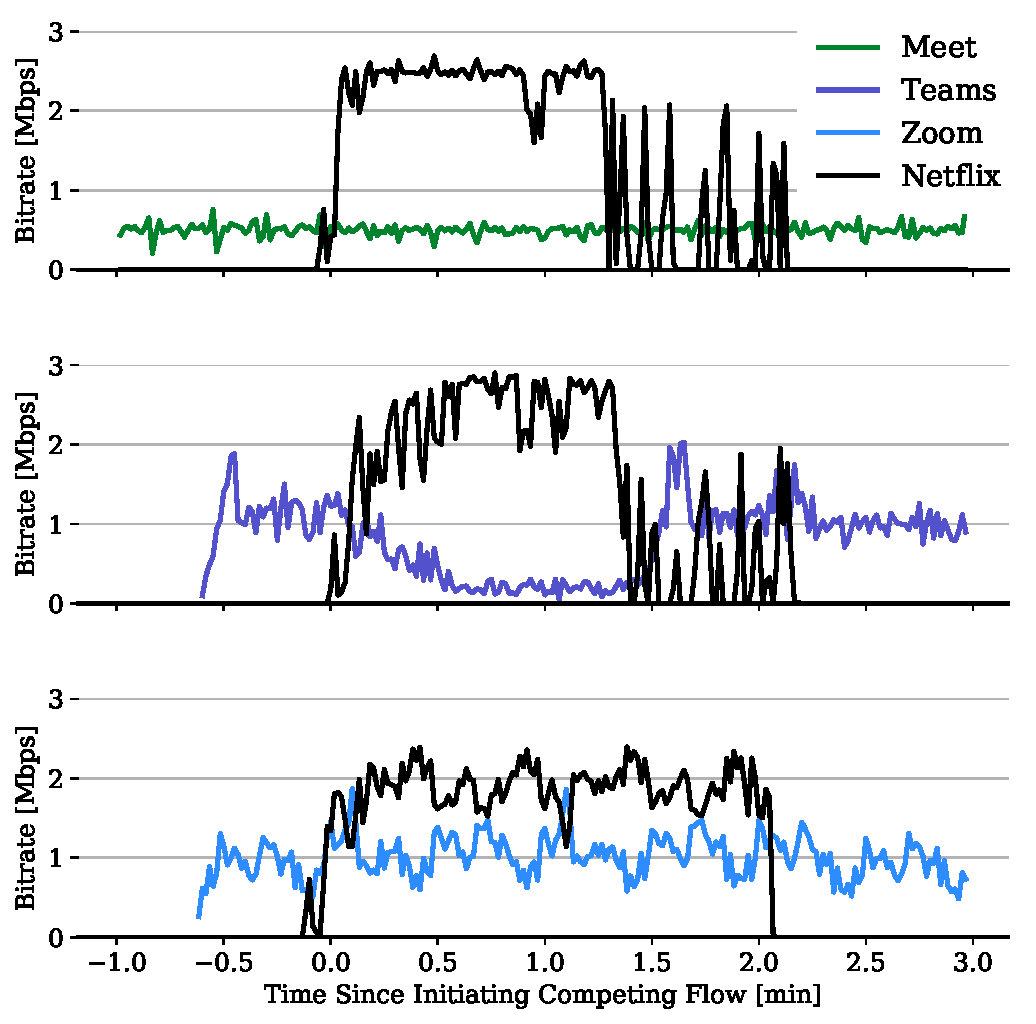
\includegraphics[width=\linewidth]{comp/netflix_time_series.pdf}
    \caption{Teams downlink bitrate when competing against non-VCA applications}
	\label{fig:ts_comp_netflix}
\end{figure}
  
Unlike VCAs, which can not buffer, the average bitrate of video streaming applications can change drastically over time. Figure \ref{fig:ts_zoom_netflix} shows how Netflix and each VCA interact over the course of the experiment. Each interaction is characterized uniquely by a given VCA. \jamie{I would move this up, to part of an `illustration.'}

First, Zoom and Meet do not back off in the presence of Netflix, and continue to receive at the same rate as before. Meet and Zoom both send at a rate lower than $50\%$ of the link capacity. But while Meet and Zoom exhibit similar behavior, their affect on Netflix is different. Because Meet receives at a lower bitrate than Zoom, Netflix maintains a high downlink bitrate as it buffers, before changing to only sporadic bursts of downlink usage. With Zoom, Netflix is not able to buffer, so maintains a constant downlink bitrate. 

Netflix also buffers when competing against Teams. But soon as Netflix is launched, Teams decreases its downlink bitrate, going as low as [insert min bitrate] Mbps. This is both undesirable for VCAs, which are sensitive to changes in bitrate, and an inefficient use of the link. Even in the face of a TCP-based application like Netflix, Teams reduces its downlink consumption. Teams only recovers to its average bitrate once Netflix has finished buffering. 
\end{comment}


% \begin{figure}[t]
%     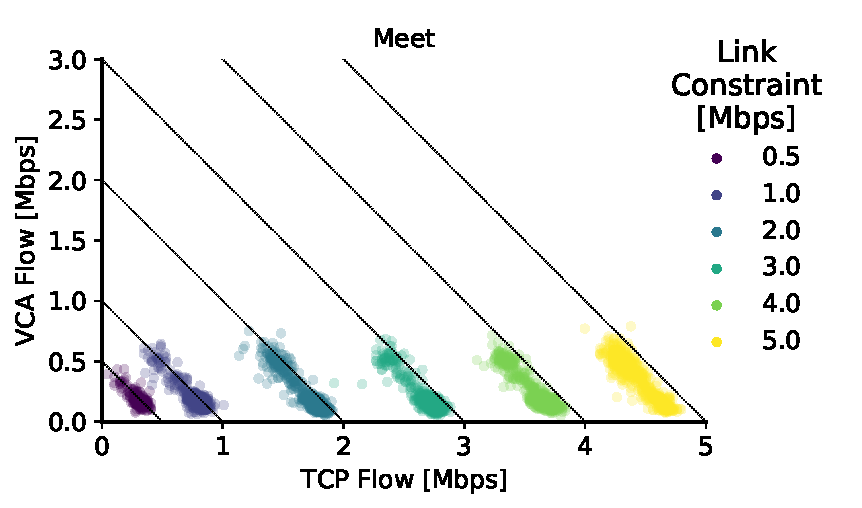
\includegraphics[width=\linewidth]{comp/meet_iperf_scatter.pdf}
%     \caption{Competition between Meet and an iperf3 TCP flow.}
% 	\label{fig:comp_meet_iperf}
% \end{figure}

% \begin{figure}[t]
%     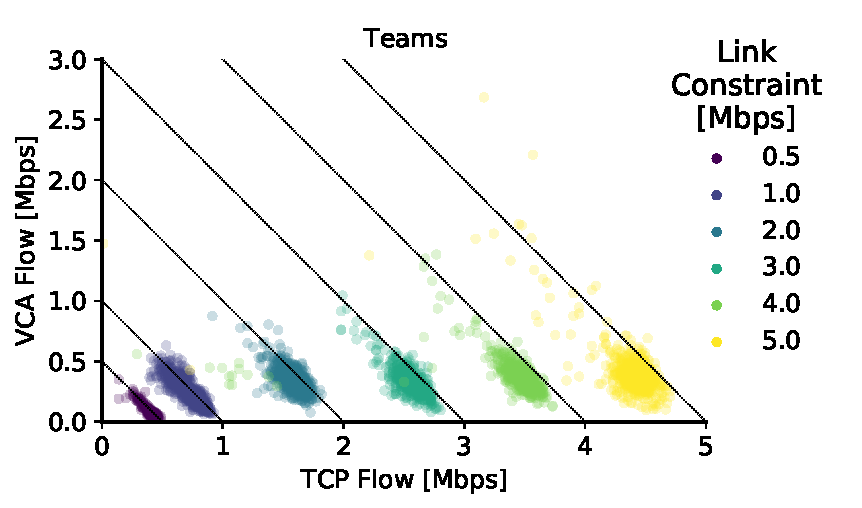
\includegraphics[width=\linewidth]{comp/teams_iperf_scatter.pdf}
%     \caption{Competition between Teams and an iperf3 TCP flow.}
% 	\label{fig:comp_teams_iperf}
% \end{figure}

\begin{comment}
Immediately noticeable is the consistency at which Meet reaches a stable bitrate.%\jamie{awkward} 
Once the link capacity reaches 1~Mbps, Meet's downlink bitrate does not increase with any further link capacity increases. Similarly, Zoom's downlink bitrate peaks at 1 Mbps, which it reaches once the link capacity is 2 Mbps. However, we observe that Teams is far less efficient in sharing the link with competing VCAs. Teams fails to reach a stable downlink bitrate, even when the link is not saturated. In Figure \ref{fig:comp_bitrates_dl}b, we see that Teams has an average downlink bitrate under 1 Mbps when competing against Zoom on a 3 Mbps link. 
We illustrate the basic setup in Figure~\ref{fig:ts_comp_netflix}, 
  pitting the VCAs against Netflix at on a link constrained to 3~Mbps.

From these flows, we construct two variables
  to reflect fairness and performance in the measured flows.
Fairness is represented 
  as the nominal flow's share of two flows constrained link.
In other words, the denominator for the ``share" is
  is the sum of the two flows rather than 
  the shaped link level.
Performance is proxied by bitrate.
Figure~\ref{fig:comp_bitrates_dl}
  displays results for all three VCAs.


Each application uses half the link in ``competition" with itself.
Competition is in evidence primarily at the low end of the domain,
  with the most severe constraints.
Table~\ref{tab:comp} shows the share
  of the flows that each VCA uses,
  at the most-constrained 0.5~Mbps level.
Here, at the low end, Zoom competes
  aggressively and effectively with all other flows:
  it consumes more than three-quarters of the link against Teams, Netflix, and iperf3, 
  and 0.72 against YouTube.
Meet is also quite aggressive at this level, 
  though Zoom ``wins" in direct competition.
Teams fares worse on very-constrained links,
  and does not even compete with the TCP flow.
  


\begin{table}
    \setlength{\tabcolsep}{3pt}
    \fontsize{10.5}{13} \selectfont
    \centering
\begin{tabular}{lcccccc}
\toprule
{} &       Meet &       Teams &        Zoom &     Netflix &     YouTube & iPerf3 \\
\midrule
Meet  &   \cbss{0.47} &  \cbsss{0.74} &   \cbss{0.43} &  \cbsss{0.76} &  \cbsss{0.71} &  \cbsss{0.72} \\
Teams &    \cbs{0.25} &   \cbss{0.41} &    \cbs{0.23} &     \cb{0.17} &    \cbs{0.26} &    \cbs{0.22} \\
Zoom  &  \cbsss{0.66} &  \cbsss{0.76} &  \cbsss{0.68} &  \cbsss{0.75} &  \cbsss{0.73} &  \cbsss{0.72} \\
\bottomrule
\end{tabular}
    \caption{Share of 0.5 Mbps link. Rows are the ``incumbent" VCAs and columns are competing applications.}
    \label{tab:comp}
\end{table}



With weaker constraints, most applications reach their nominal bitrates
  and the ratios in the upper panels of Figure~\ref{fig:comp_bitrates}
  simply show the ratio of their bandwidth demands.
For example, 
  the low VCA shares with respect to iperf at weak constraint
  simply illustrates the "inexhaustible" demand of a TCP flow,
  whereas link share's of Zoom vs Meet or Meet vs Zoom 
  at link capacity of 5 Mbps (0.4 or 0.6) simply 
  reflect different nominal bandwidths.
As already shown, in the time series plots, there is some subtlety in the timing of competition.
Video streaming services (YouTube and NetFlix)
  can and do buffer, ifthe bandwidth is high enough.
This means that they may not compete most of the time.
The VCAs and the iPerf3 TCP flows on the other hand, 
  are continuous, though only iPerf3 has inexhaustible demand.
The VCAs seem to ``test" the bandwidth early in the call, 
  and the fist moments may not illustrate their long-term strategies.
This is analogous to TCP ``slow-start,"
  but appears to be much slower.

The lower panels of Figure~\ref{fig:comp_bitrates} show
  the VCAs' bitrates, in competition.
Again, Zoom is quick out of the gate, and 
  achieves over 90 of nominal link bitrate,
  for constraints weaker than 2 Mbps.
On the other hand, Teams does not achieve full bitrate
  below 5~Mbps;
  \jamie{at 10~Mbps, it achieves a flow of X}.
Depending on the flow, Meet's used bitrate saturates
  when the shared link has capacity greater than 3 Mbps.
The same is true for Zoom, though its plateau is higher and noisier.
  
\jamie{We start getting repetitive here}
 Looking first at how Meet competes with other VCAs, it uses slightly less than Zoom but dominates Teams. Meet is also remarkably fair when competing with another Meet flow, splitting the available link capacity almost exactly evenly. Against TCP applications, Meet commands roughly $75\%$ of the available link capacity at the 0.5 Mbps shaping level. 

While not quite as consistent as Meet, Zoom nevertheless shares the link in a similar manner regardless of the competing application. At low link capacities, Zoom uses up to [X] \% of the the available bandwidth. By [X] Mbps, its downlink bitrate remainly roughly the same. 

This consistency manifests differently in how Teams competes. 
Where Zoom and Meet aggressively use the available link capacity at low bandwidths, Teams backs off, in almost all cases using less than $25\%$ of the available bandwidth on a 0.5 Mbps downlink connection. Consider first how Teams behaves with other VCAs. While still dominated at the low end, as the link capacity increases and Zoom and Meet reach a stable downlink bitrate, Teams begins to also increase its downlink bitrate. Notice, however, that even at a 5 Mbps link capacity, Teams's downlink bitrate does not exceed 1.25 Mbps. Looking next at how Teams competes with the TCP-based applications, we observe even more startling behavior. When competing against Netflix and the iPerf3 flow, the downlink bitrate never exceeds 0.25 Mbps. This is especially inexpedient given the sensitivity of VCAs to drops in bandwidth and the goal of equitably sharing the link.  \jamie{Maybe careful here?  This isn't necessarily how peaky ``TCP applications" fare, it's how a single continuous flow fares.  It may be that individual TCP requests can get through fine, cf buffer bloat etc.}
\end{comment}
